
\documentclass[a4paper]{article}
\usepackage[pdftex]{graphicx,color}  % ab: for xfig pdf export
%\usepackage{showframe}
% minted
\usepackage{minted}
\usemintedstyle{lovelace}
\definecolor{bg}{rgb}{0.95,0.95,0.95}
\definecolor{bg_shell}{rgb}{0.95,0.95,1.00}
%\newminted[python]{python}{bgcolor=bg, frame=lines}
\newminted[python]{python}{frame=lines}
%\AfterEndEnvironment{minted}{\par\noindent}
%\makeatletter
%\patchcmd{\minted@colorbg}{\noindent}{\medskip\noindent}{}{}
%\apptocmd{\endminted@colorbg}{\par\medskip}{}{}
%\makeatother




%\addtolength{\topmargin}{-2cm}
\addtolength{\textheight}{1cm}
%\addtolength{\textwidth}{1cm}
%\addtolength{\oddsidemargin}{-0.5cm}



\title{The Accelerator\\[1ex]\large{Technical Overview}}
%\\[1ex]\large{Processing One Billion Lines of
%    Data per Second on a Single PC}\\\Large{--- DRAFT @7cb02a8---}}
\author{\tiny{A.\,Berkeman, C.\,Drougge, and S.\,H\"orberg}}
\date{}

\begin{document}
\maketitle
\thispagestyle{empty}

\clearpage
\tableofcontents
\thispagestyle{empty}

%\begin{figure}[h]
%  \centering
%  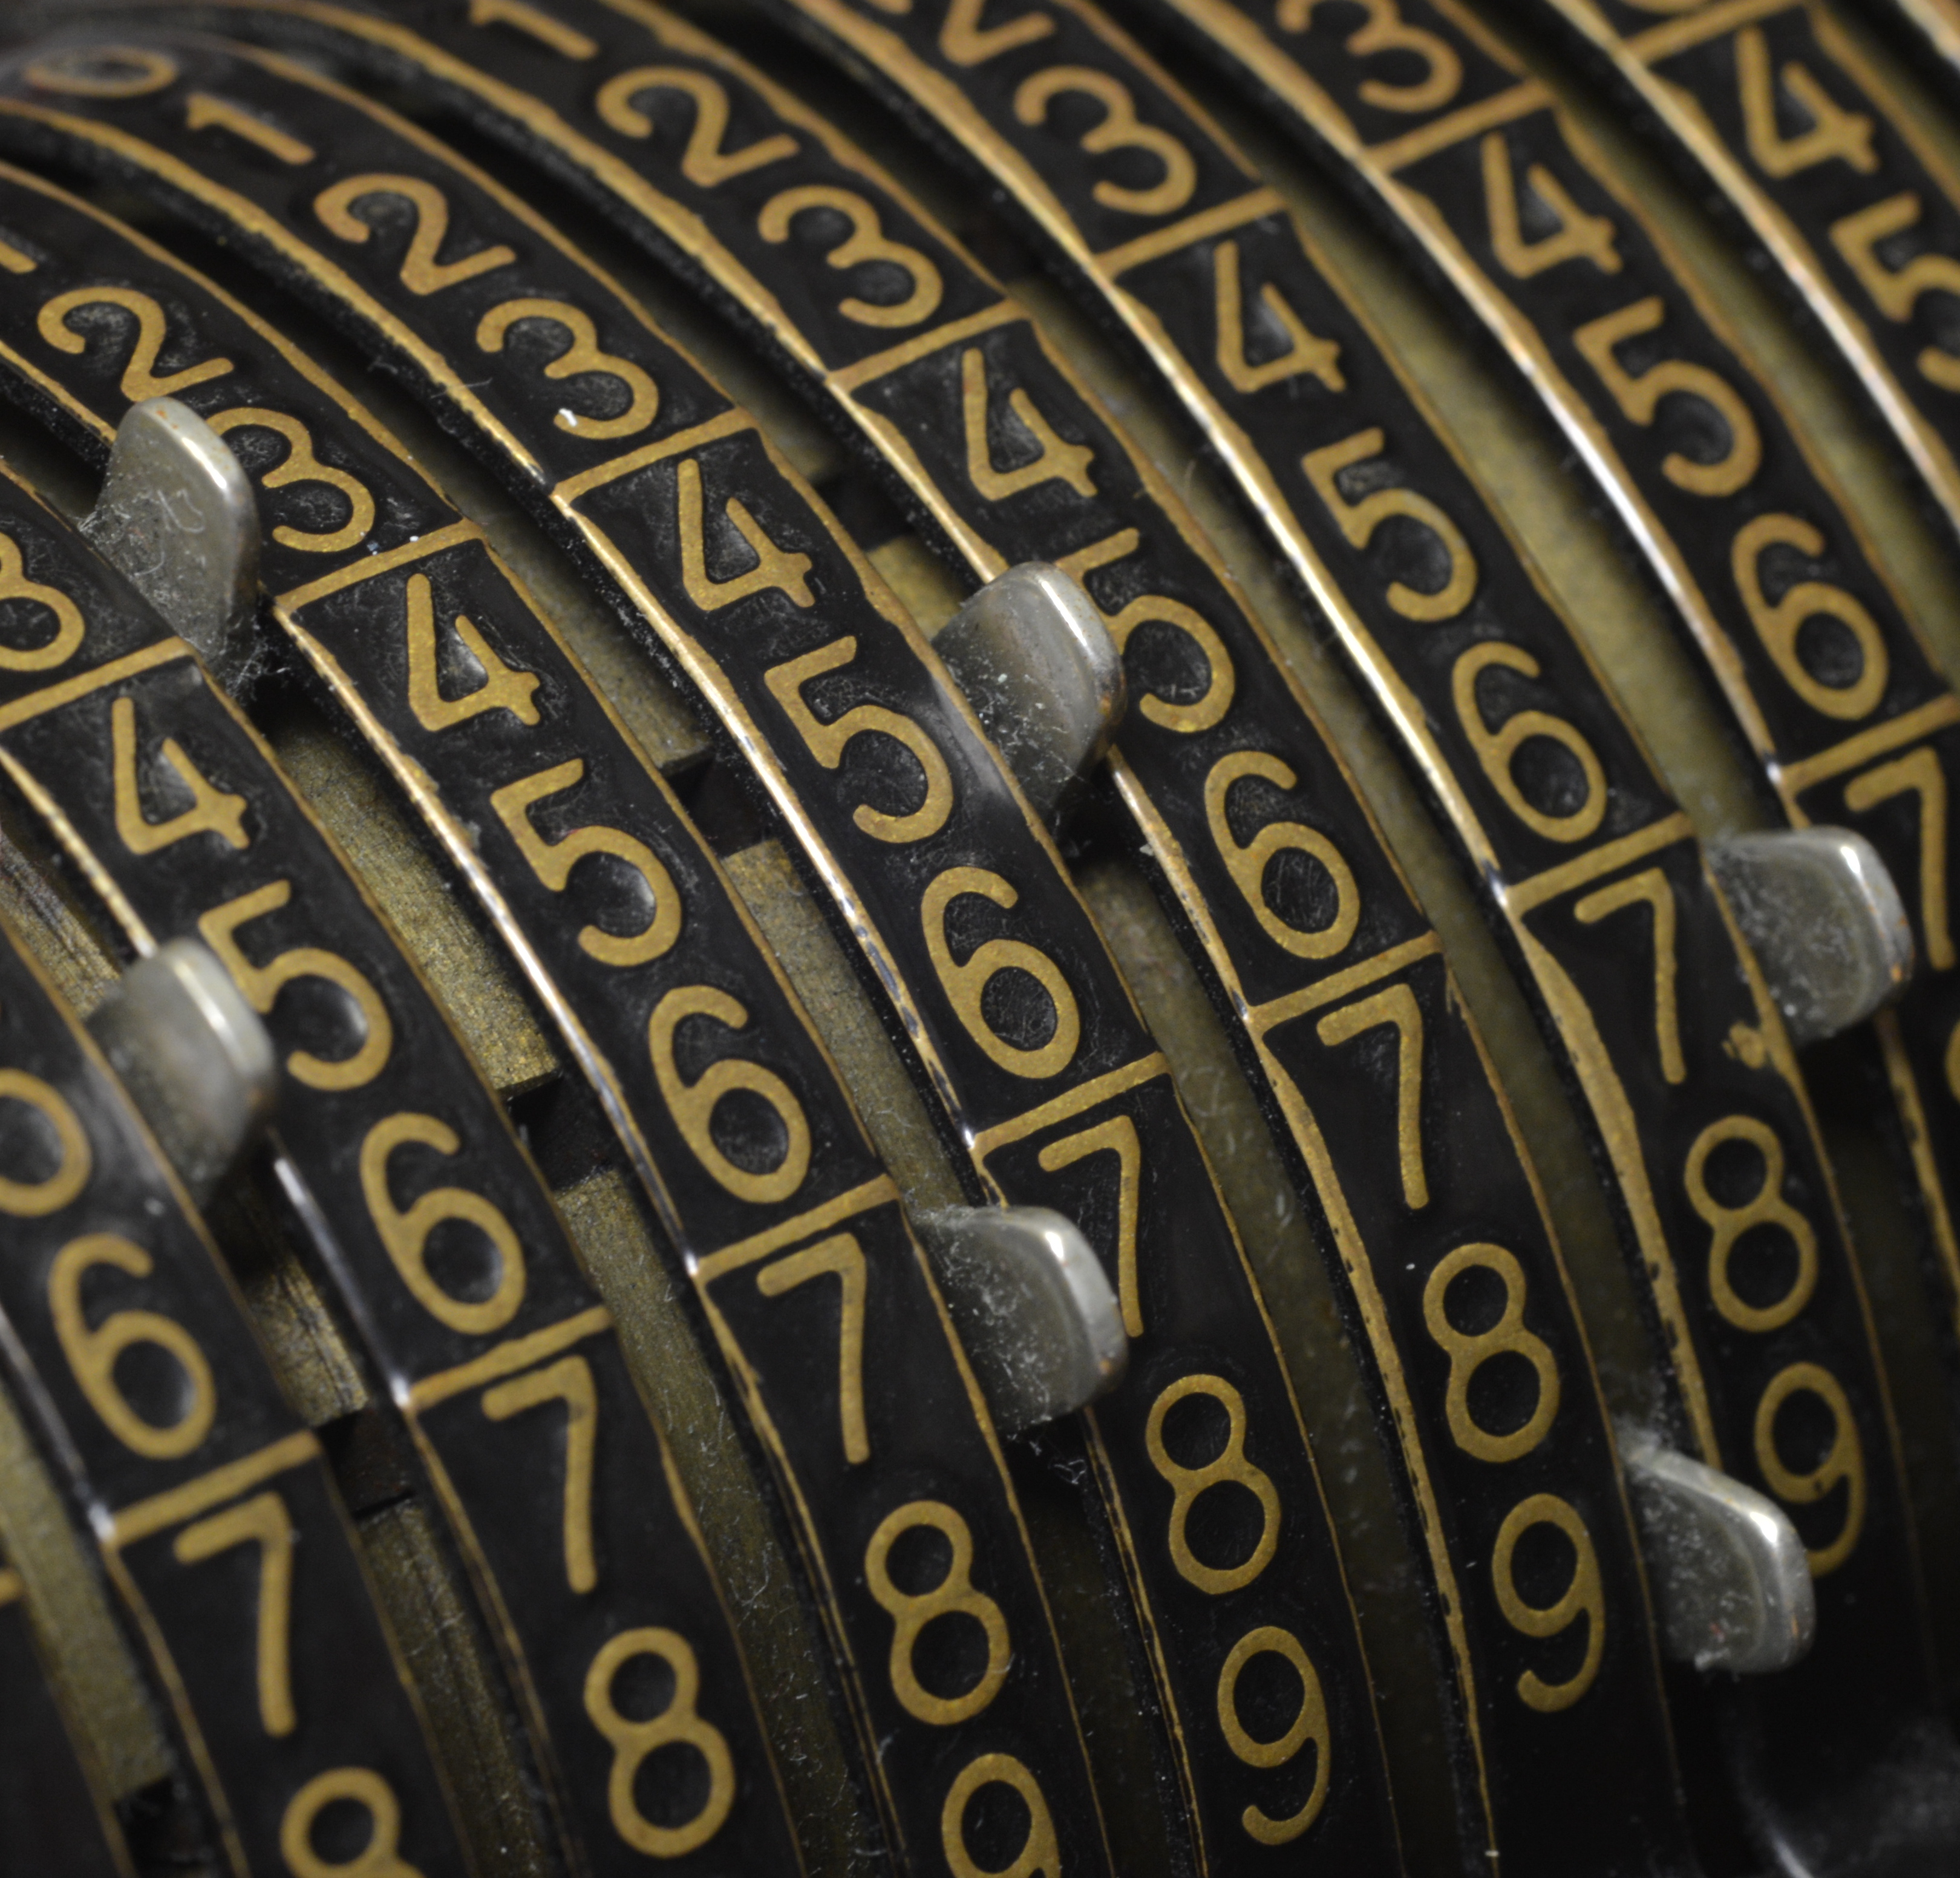
\includegraphics[width=11cm]{odhner_square.jpg}
%\end{figure}

%% \begin{figure}[h]
%%   \begin{center}
%%     \input{figures/test.pdftex_t} %the difference is just this part
%%     \caption{caption here}
%%     \label{figure:example}
%%   \end{center}
%% \end{figure}



% Your 1-page abstract should include:

% Motivation: Why do we care about the problem and the results?

% Problem statement: What problem are you trying to solve? What is
%   the scope of your work (a generalized approach, or for a specific
%   situation)?

% Approach: How did you go about solving or making progress on
%   the problem? Did you use simulation, analytic models,
%   prototype construction, or analysis of field data for an
%   actual product? What was the extent of your work (did you look
%   at one application program or a hundred programs in twenty
%   different programming languages?) What important variables did
%   you control, ignore, or measure?

% Results: What's the answer?
%   Conclusions: What are the implications of your answer? Is
%   it going to change the world (unlikely), be a significant
%   ``win'', be a nice hack, or simply serve as a road sign
%   indicating that this path is a waste of time (all of the
%   previous results are useful). Are your results general,
%   potentially generalizable, or specific to a particular
%   case?
            

%% \emph{
%%  teaser om hur coola grejer man kan göra innan vi börjar med triviala
%%  exempel...  ``Så, för att förstå hur det är möjligt måste vi börja
%%  med...'', typ
%% }\\

%% \emph{Maste namna workspace eller om det heter workdir}\\

%% \emph{Maste namna python}\\


%% \subsection*{What It Is}
%% The Expertmaker Accelerator is a tool for processing big data.  It has
%% a small footprint and low overhead, and provides a number of
%% interesting features, most notably very fast data access and a novel
%% scheme to store, retrieve, and reuse computations.  It has been used
%% in commercial projects since 2012.

%% \subsection*{Background}
%% vad den anvants till, hur den utvecklats osv

%% \subsection*{Motivation and Approach}
%% Processing big data is potentially both time consuming and resource
%% hungry.  This is addressed in the Accelerator design by the following
%% two principles:
%% \begin{itemize}
%% \item[1.] Modern computers are very powerful.\\ The Accelerator has
%%   very vast data streaming from disk to CPU cores.  Critical parts are
%%   written in the C programming language, and effort has been spent to
%%   come close to the theoretical performance limits set by modern
%%   hardware.
  
%% \item[2.] Results are valuable, they should be easy to retrieve and
%%   re-use.\\ The Accelerator connects each computed result to the
%%   source code that was running, the input data used, and the set of
%%   input parameters.  This connection makes it possible for the
%%   Accelerator to automatically retrieve results instead of
%%   re-computing them, which saves time.  It also brings full
%%   transparency in that all work can be trivially traced back to its
%%   origins.
%% \end{itemize}



















%%%%%%%%%%%%%%%%%%%%%%%%%%%%%%%%%%%%%%%%%%%%%%%%%%%%%%%%%%%%%%%%%%%%%%%%%%%%%%%%
\clearpage
\section{Introduction}
The Accelerator is a tool for fast data processing.  Typical
applications include data analysis as well as live production systems
for varous data processing tasks, such as recommendation systems, and
more.  It has a small footprint and runs on laptops as well as rack
servers.

It was first used in 2012, and has been continuously developed and
improved since.  In 2016, it was aquired by Ebay, who decided to open
source it early 2018.



\subsection{History}
The Accelerator has been in use since 2012 in a number of different
projects.  Most project have been related to data analysis, some to
optimisation, and some projects have been live-running recommendation
systems for years.  The Accelerator has evolved from being the core of
these projects.

Data set sizes in these projects range from a few hundred lines up to
several tens of billions rows with multiple columns.  The number of
items in a dataset used in a live system was well above $10^{11}$, and
this was handled with ease on a \emph{single} 32 core computer.


\subsection{Authors and Git Repository}
The authors are Anders Berkeman, Carl Drougge, and Sofia H\"orberg.
About 1500 commits have been removed to clean up the open version of
the code base.  Extensive testing has been done by Stefan Hakonsson.


\clearpage
\section{Overview}




\subsection{Main Design Goals}
The Accelerator is developed bottom up for high performance and
simplicity, and the main design goals are
\begin{itemize}
\item[] Parallel processing should be made simple.  Modern computers
  come with several cores, it should be straightforward to make use of
  them.
\item[] Make access to data really fast.  It should be possible to
  process large datasets, even on commodity hardware.
\item[] Never recompute old results, always recycle jobs, when
  possible.  Also, sharing results between multiple users should be
  effortless.
\end{itemize}
In addition, the Accelerator is designed to be used in all levels of a
project, including data analysis, algorithm development, as well as
production.  Using the same tool for analysis and production closes
the loop between input and output, making it really simple to analyse
and get insights from the whole system.

\subsection{High Level View}

The Accelerator is a client-server based application, and the current
setup is as follows.

\begin{figure}[h!]
  \begin{center}
    \section{Jobs:  Executing Code}
The basic operation of the Accelerator is to execute small programs
called \textsl{methods}.  In a method, some reserved function names
are used to execute code sequentially or in parallel and to pass
parameters and results.  A method that has completed execution is
called a \textsl{job}.

The Accelerator keeps a record of all jobs that have been run.  It
turns out this is very useful for avoiding unnecessary re-computing
and instead rely on previosly computed results.  This does not only
speed up processing and encourage incremental design, but also makes
it transparent which code and which data was used for any particular
result, thus reducing uncertainty.

In this section, we'll look at basic job running, result sharing, and
parameters.


\subsection{Basic Job Running:  ``Hello, World''}

Let's begin with a simple ``hello world'' program.  We create a method
with the following contents
\begin{python}
def synthesis():
    return ``hello world''
\end{python}
This program does not take any input parameters.  It just returns a
string and exits.  Running methods on the Accelerator is further
explained in section~\ref{sec:urd}.

When execution of the method is completed, a single link, called a
\texttt{jobid} is the only thing that is returned to the user.  The
jobid points to a directory where the result from the execution is
stored, together with all information that was needed to run the job
plus some profiling information.

If we try to run the job again it will not execute, simply because the
Accelerator remembers the job has been run in the past.  Instead of
running the job again, it immediately returns the jobid pointing to
the previous run.  This means that from a user's perspective, there is
no difference between job running and job result recalling!  In order
to have the job executing again, we have to change either the source
code or input parameters.

Figure~\ref{fig:execflow-hello-world} illustrates the dispatch of the
\texttt{hello\_world} method.  The created jobid is called
\texttt{test-0}, and corresponding directory information is shown in
green.  The job directory contains several files, of which the most
important ones right now are
\begin{itemize}
\item[] \texttt{setup.json}, which contains job information; and
\item[] \texttt{result.pickle}, that contains the returned data.
\end{itemize}

\begin{figure}[h!]
  \begin{center}
    \input{figures/job0.pdftex_t}
    \caption{A simple hello world program, represented as graph and
      work directory.}
    \label{fig:execflow-hello-world}
  \end{center}
\end{figure}






\subsection{Linking Jobs}
Assume that the job that we just run was computationally expensive,
and that it returned a result that we'd like to use as input to further
processing.

To keep things simple, we demonstrate the principle by creating a
method that just reads and prints the result from the previous job to
\texttt{stdout}.  We create a new method \texttt{print\_result}, that
goes like this

\begin{python}
import blob

jobids = {'hello_world_job',}

def synthesis():
    x = blob.load(jobid=jobids.hello_world_job)
    print(x)
\end{python}

This method expects the \texttt{hello\_world\_job} input parameter to
be provided at execution time, and we will see in section~\ref{xxx}
how to do this.  The method then reads the result from the provided
jobid and assigns it to the variable \texttt{x}, which is then printed
to \texttt{stdout}.  Note that this method does not return anything.
Figure~\ref{fig:execflow-print-result} illustrates the situation.
Note the direction of the arrow - The second job, \texttt{test-1} had
\texttt{test-0} as input parameter, but \texttt{test-0} does not know
of any jobs run in the future.

\begin{figure}[h!]
  \begin{center}
    \input{figures/job0job1.pdftex_t}
    \caption{Jobid \texttt{test-0}, is used as input to the
      \texttt{print\_result} job.}
    \label{fig:execflow-print-result}
  \end{center}
\end{figure}

\subsection{Job Execution Flow and Result Passing}

There are three functions in a method that are called from the
Accelerator when a method is running, and they are \texttt{prepare()},
\texttt{analysis()}, and \texttt{synthesis()}.  All three may exist in
the same method, and at least one is required.  When the method
executes, they are called one after the other.
\begin{itemize}
\item[] \texttt{prepare()} is executed first.  The returned value is
  available in the variable \texttt{prepare\_res}.
\item[] \texttt{analysis()} is run in parallel processes, one for each
  slice.  It is called after completion of \texttt{prepare()}.  Common
  input paramerers are \texttt{sliceno}, holding the number of the
  current process instance, and \texttt{prepare\_res}.  The return
  value for each process becomes available in the
  \texttt{analysis\_res} variable.
\item[] \texttt{synthesis()} is called after the last
  \texttt{analysis()}-process is completed.  It is typically used to
  aggregate parallel results created by \texttt{analysis()} and takes
  both \texttt{prepare\_res} and \texttt{analysis\_res} as optional
  parameters.  The latter is an iterator of the results from the
  parallel processes.
\end{itemize}
Figure~\ref{fig:prepanasyn} shows the execution order from top to
bottom, and the data passed between functions in coloured branches.
\texttt{prepare()} is executed first, and its return value is
available to both the \texttt{analysis()} and \texttt{synthesis()}
functions.  There are \texttt{slices} (a configurable parameter)
number of parallel \texttt{analysis()} processes, and their output is
available to the \texttt{synthesis()} function, which is executed
last.

Return values from any of the three functions may be stored in the
job's directory making them available to other jobs.


\begin{figure}[h!]
  \begin{center}
    \input{figures/prepanasyn.pdftex_t}
    \caption{Execution flow and result propagation in a method.}
    \label{fig:prepanasyn}
  \end{center}
\end{figure}
\subsection{Job Parameters}


We've seen how jobids from completed jobs can be used as input to new
jobs.  Jobid parameters is one of three kinds of input parameters that
a job can take.  Here the input parameters are summarised:
\begin{itemize}
\item[] \texttt{jobids}, a set of identifiers to previously executed jobs;
\item[] \texttt{options}, a dictionary of options; and
\item[] \texttt{datasets}, a set of input \textsl{datasets}, explained later.
\end{itemize}
See Figure~\ref{fig:execflow}.  Parameters are entered as global
variables early in the method's source.



\subsubsection*{The Params Variable}
A job's parameters are always available in the \texttt{params}
variable.  The \texttt{params} variable is make available by adding it
as input to \texttt{prepare()}, \texttt{analysis()}, or
\texttt{synthesis()}, like this
\begin{python}
def synthesis(params):
    print(params)
\end{python}
Accessing the \texttt{params} variable for \textsl{another} job is
done like this
\begin{python}
jobids = {'thejob',}

def synthesis():
    print(jobids.thejob.params)
\end{python}
it turns out it can be very useful to know for example which datasets
another job has been processing, and so on.

Apart from the input parameters, the \texttt{params} variable also
gives access to more information about the job and the current
Accelerator setup, such as the total number of slices, the random
seed, the hash of the source code, and method execution start time.


\begin{figure}[h!]
  \begin{center}
    \input{figures/execflow.pdftex_t}
    \caption{Execution flow of a method.  The method takes optionally
      three kinds of parameters: \texttt{options}, \texttt{jobids},
      and \texttt{datasets}.}
    \label{fig:execflow}
  \end{center}
\end{figure}


\subsubsection*{Input parameter \texttt{jobids}}
The \texttt{jobids} parameter is a set containing any number of input
jobids.  For example
\begin{python}
jobid = {'sales_stats', 'overhead_stats',}
\end{python}
When a method is to be executed, actual links to jobs, i.e.\ jobids,
are passed using these parameters.


\subsubsection*{Input parameter \texttt{options}}
Options are supplied as a dictionary and is very flexible in typing.  For example
\begin{python}
options = dict(
    name = 'alice',
    defaultnames = set('alice', 'bob'),
    param1 = 1,
    param2 = float,
)
\end{python}
Here, values are defaults, so \texttt{param1} is default set to 1,
while a floating point value must be supplied to \texttt{param2}.

\subsubsection*{Input parameter \texttt{datasets}}
Datasets will be described in more details later, and the
\texttt{datasets} parameter is similar to the \texttt{jobids}
parameter.




%%%%%%%%%%%%%%%%%%%%%%%%%%%%%%%%%%%%%%%%%%%%%%%%%%%%%%%%%%%%%%%%%%%%%%%%%%%%%%%%

\section{Datasets: Storing Data}

The \texttt{dataset} is the Accelerator's default storage type for
small or large quantities of data, designed for parallel processing
and high performance.  Datasets are built on top of jobs, so
\emph{datasets are created by methods and stored in job directories,
  just like any job result.}

Internally, data in a dataset is stored in a row-column format, and is
typically \emph{sliced} into a fixed number of slices to allow
efficient parallell access.  Columns are accessed independently.
Furthermore, datasets may be \textsl{hashed}, so that slicing is based
on the hash value of a given column.  In many practical applications,
hashing makes parallel processes independent, minimising the need for
complicated merging operations.  This is explained further in
section~\ref{sec:dataset-hashing}.



\subsection{Importing Data}

Let's have a look at the common operation of \textsl{importing},
i.e.\ creating a dataset from a file.  See
figure~\ref{fig:dataset_csvimport}.

\begin{figure}[h!]
  \begin{center}
    \input{figures/import_file1.pdftex_t}
    \caption{Importing \texttt{file0.txt}.}
    \label{fig:dataset_csvimport}
  \end{center}
\end{figure}

\noindent The standard method \texttt{csvimport}, is designed to parse
a pletoria of ``comma separated values''-file formats and store the
data as a dataset.  The method takes several input options, where the
file name is mandatory.  The created dataset is stored in the
resulting job, and the name of the dataset will by default be the
jobid plus the string \texttt{default}.  For example, if the
\texttt{csvimport} jobid is \texttt{imp-0}, the dataset will be
referenced by \texttt{imp-0/default}.  In this case, and always when
there is no ambiguity, the jobid alone (\texttt{imp-0}) could be used
too.





\subsection{Linking Datasets, Chaining}

Just like jobs can be linked to eachother, datasets can link to
eachother too.  Since datasets are build on top of jobs, this is
straightforward.  Assume that we've just imported \texttt{file0.txt}
into \texttt{imp-0/default} and that there is more data like it stored
in \texttt{file1.txt}.  We can import the latter file and supply a
link to the previous dataset, see
figure~\ref{fig:dataset_csvimport_chain}.

\begin{figure}[h!]
  \begin{center}
    \input{figures/import_file0file1.pdftex_t}
    \caption{Chaining the import of \texttt{file1.txt} to the previous
      import of \texttt{file0.txt}.}
    \label{fig:dataset_csvimport_chain}
  \end{center}
\end{figure}

\noindent The \texttt{imp-1} (or \texttt{imp-1/default}) dataset
reference can now be used to access all data imported from both files!

Linking datasets containing related content is called \emph{chaining},
and this is particularly convenient when dealing with data that grows
over time.  Good example are all kind of \emph{log} data, such as logs
of transactions, user interactions, etc.

Using chaining, we can extend datasets with more rows just by linking,
which is a very lightweight operation.



\subsection{Adding New Columns to a Dataset}
We have seen how easy it is to add more lines to data to a dataset
using chaining.  The only thing that needs to be done is to set a
link, so the overhead is minimal.

Now we'll see that is it equally simple to add new columns to an
existing dataset.  Adding columns is also a common operation and the
Accelerator handles it efficiently using links.

The idea is very simple.  Assume that we have a ``source'' dataset to
which we want to add a new column.  We create a new dataset containing
\textsl{only} the new column, and while creating it we instruct the
Accelerator to link the source dataset to the new column.

Accessing the new one-column dataset will transparently access all the
data in the source dataset too, making it indistinguishable from a
single dataset.  See Figure~\ref{fig:dep_dataset_append_column}.

\begin{figure}[h!]
  \begin{center}
    \input{figures/dataset_append_column.pdftex_t}
    \caption{caption here}
    \label{fig:dep_dataset_append_column}
  \end{center}
\end{figure}





\subsection{Multiple Datasets in a Job}

We've seen that datasets are created by methods and stored in job
directories.  Typically, a method creates a single dataset in the job
directory, but there is no limit on how many datasets that could be
created and stored in a single job directory.  This leads to some
interesting applications.

One application where it is convenient to create multiple datasets in
a job is when splitting data into subsets based on some condition.
For example, assume that we want to separate a dataset into two
disjoint datasets based on a column storing a boolean value.  See
Figure~\ref{fig:dep_dataset_csvimport_chain}.

\begin{figure}[h!]
  \hspace{1cm}
  \input{figures/filter_dataset.pdftex_t}
  \caption{\texttt{job-1} separates the dataset
    \texttt{job-0/default} into two new datasets, named
    \texttt{job-1/train} and \texttt{job-1/test}.}
  \label{fig:dep_dataset_csvimport_chain}
\end{figure}

The figure shows how \texttt{job-1} has created two datasets,
\texttt{job-1/train} and \texttt{job-1/test}, based on the input
dataset \texttt{job-0/default}.  A third job, \texttt{job-2} is then
accessing the \texttt{job-1/train} dataset.  (Note that \texttt{job-1}
does not have a \texttt{default} dataset.)



%% Short repetition on the direction of the arrow.  \texttt{job\_1}
%% filtered the \texttt{dataset} from \texttt{job\_0}.  So if we take a
%% look at \texttt{job\_1} and wonder where the input data is, we just
%% follow the link back to \texttt{job\_0}.  If this job is an import, it
%% will hold the name of the file that was imported.  If not, it will
%% link back to another job, and so on, all the way down to the source of
%% the dataset.  So there is full tracking and easy observability of
%% everything that relates to job execution in the Accelerator.

\emph{
  Let us look at an example of when such dataset splitting
  makes sense, and how it relates to the design methodology that the
  Accelerator is based upon.  Assume that we have a (perhaps large)
  dataset that we want to split into, say, a training set and a
  validation set.  Even if one set is small, it makes sense to split the
  dataset into two disjoint sets.  This way, we ``physically'' separate
  the data into two sets, while keeping all the data in the same place.
  This is good for transparency reasons, and any method following the
  split may iterate over both subsets to read the complete data.
}


\subsection{Parallel Dataset Access and Hashing}
As shown in detail in section~\ref{xx}, data in datasets are stored in
multiple files, allowing for fast parallel reads.  The parameter
\texttt{slices} (\ref{xx}) determines how many slices that the dataset
should be partitioned into.  This parameter also sets the number of
parallel \texttt{analysis}-processes, so that each \texttt{analysis}
process operates on a unique slice of the dataset.

Datasets can be partitioned, sliced, in different ways.  One obvious
way is to use round robin, where each consecutive data row is written
to the next slice, modulo the number of slices.  This leads to
datasets with approximately equal number of rows per slice.  Another
alternative to slicing is to slice based on the hash value of a
particular column's values.  Using this method, all rows with the same
value in the hash column end up in the same slice.  This is efficient
for some parallel processing tasks.




\subsection{Dataset Column Types}
\label{sec:dataset-typing}
There are a number of useful types available for dataset columns.
They include floating and integer point numbers, booleans, timestamps,
several string types, and json types.  Several of these types are
designed to make importing data from text files straightforward,
without parse errors, overflows etc.



\subsection{Dataset Attributes}
The dataset has a number of attributes associated with it, such as
shape, number of rows, column names and types, and more.
An attribute is accessed like this
\begin{python}
datasets = ('source',)
def synthesis():
    print(datasets.source.shape)
\end{python}



%%%%%%%%%%%%%%%%%%%%%%%%%%%%%%%%%%%%%%%%%%%%%%%%%%%%%%%%%%%%%%%%%%%%%%%%%%%%%%%%

\section{Iterators: Working with Data}

Data in a dataset is typically accessed using an \emph{iterator} that
reads and streams one dataset slice at a time to a CPU core.  In this
section, we'll have a look at iterators for reading data, how to take
advantage of slicing to have parallel processing, and how to
efficiently create datasets.

\subsection{Iterator Basics}

Assume that we have a dataset with a column containing movie titles
named \texttt{movie}, and we want to know the ten most frequent
movies.  Consider the following example of a complete method
\begin{python}
from collections import Counter
datasets = ('source',)

def synthesis():
    c = Counter(movie for movie in datasets.source.iterate(None, 'movie'))
    print(c.most_common(10))
\end{python}
This will print the ten most common movie titles and their
corresponding counts in the \texttt{source} dataset.  The code will
run on a single CPU core, because of the \texttt{synthesis} function,
which is called only once.  The \texttt{iterate} (class-)method
therefore has to read through all slices, one at a time, in a serial
fashion, and this is reflected by the first argument to the iterator
being \texttt{None}.


\subsection{Parallel Execution}
The Accelerator is much about parallel processing, and since datasets
are sliced, we can modify the above program to execute in parallel by
doing the following modification
\begin{python}
def analysis(sliceno):
    return Counter(movie for movie in datasets.source.iterate(sliceno, 'movie'))

def synthesis(analysis_res)
    c = analysis_res.merge_auto()
    print(c.most_common(10))
\end{python}
Here, we run \texttt{iterate} inside the \texttt{analysis()} function.
This function is forked once for each slice, and the argument
\texttt{sliceno} will contain an integer between zero and the number
of slices minus one.  The returned value from the analysis functions
will be available as input to the synthesis function in the
\texttt{analysis\_res} Python iterable.  It is possible to merge the
results explicitly, but the iterator comes with a rather magic method
\texttt{merge\_auto()}, which merges the results from all slices into
one based on the data type.  It can for example merge
\texttt{Counter}s, \texttt{set}s, and composed types like
\texttt{set}s of \texttt{Counter}s, and so on.


\subsection{Iterating over Several Columns}
Since each column is stored independently in a dataset, there is no
overhead from reading a subset of a dataset's columns.  In the
previous section we've seen how to iterate over a single column using
\texttt{iterate}.  Iterating over more columns is straightforward by
feeding a list of column names to \texttt{iterate}, like in this
example
\begin{python}
from collections import defaultdict
datasets = {'source',}

def analysis(sliceno):
    user2movieset = defaultdict(set)
    for user, movie in datasets.source.iterate(sliceno, ('user', 'movie')):
    user2movieset[user].add(movie)
    return user2movieset
\end{python}
This example creates a lookup dictionary from users to sets of movies.
It is also possible to iterate over all columns by specifying an empty
list of columns or by using the value \texttt{None}.
\begin{python}
...
def analysis(sliceno):
    for columns in datasets.source.iterate(sliceno, None):
    print(columns)
    break
\end{python}
This example will print the first row for each slice of a dataset and
then exit.


\subsection{Iterating over Dataset Chains}

Previously, we've seen how to iterate over a single dataset using
\texttt{iterate}.  There is a corresponding function,
\texttt{iterate\_chain}, that is used for iterating over chains of
datasets.  This function takes a number of arguments, such as
\begin{itemize}
\item[] \texttt{length}, i.e.\ the number of datasets to iterate over.
  By default, it will iterate over all datasets in the chain.
\item[] \texttt{callbacks}, functions that can be called before and/or
  after each dataset in a chain.  Very useful for aggregating data
  between datasets.
\item[] \texttt{stop\_jobid} which stops iterating at a certain jobid.
  This jobid could be from \textsl{another} job's parameters, so we
  can for example iterate exactly over all new datasets not covered by
  a previous job.

\item[] \texttt{range}, which allows for iterating over a range of
  data.
\end{itemize}
The \texttt{range} options is based on the max/min values stored for
each column in the dataset.  Assuming that the chain is sorted, one
can for example set \mintinline{python}{range={timestamp, ('2016-01-01', '2016-01-31')}}
in order to get rows within the specified range only.  The %
\texttt{range} is quite costly, since it requires each row in the
dataset chain with dates within the range to be checked against the
range criterion.  Therefore, there is a \texttt{sloppy} version that
iterates over complete datasets in the chain that contains at least
one row with a date within the range.  This is useful, for example, to
very quickly produce histograms or plots of subsets of the data.


\subsection{Asserting the Hashlabel}
Depending on how the parallel processing is implemented in a method,
some methods will only work if the input datasets are hashed on a
certain column.  To make sure this is the case, there is an optional
\texttt{hashlabel} parameter to the iterators that will cause a
failure if the supplied column name does not correspond to the
dataset's hashlabel.

It is also possible to have the iterate re-hash on-the-fly.  In
general this is not recommended, since there is a
\texttt{dataset\_rehash} method that does the same and stores the
result for immediate re-use.  Using \texttt{dataset\_rehash} will be
much more efficient.

\subsection{Dataset Translators and Filters}

The iterator may perform data translation and filtering on-the-fly
using the \texttt{translators} and \texttt{filters} options.  Here is
an example of how a dictionary can be fed into the iterator to map a
column
\begin{python}
mapper = {2: ``HUMANLIKE'', 4: ``LABRADOR'', 5: ``STARFISH'',}
for animal in datasets.source.iterate_chain(sliceno, \
  ``NUM_LEGS'', translator={``NUM_LEGS'': mapper,}):
    ...
\end{python}
This will iterate over the \texttt{NUM\_LEGS} column, and map numbers
to strings according to the \texttt{mapper} dict.

Filters work similarly.


    \caption{}
    \label{fig:overview}
  \end{center}
\end{figure}






\clearpage
\section{Executing Code: Jobs}
The basic operation of the Accelerator is to execute small programs
called \textsl{methods}.  In a method, some reserved function names
are used to execute code sequentially or in parallel and to pass
parameters and results.  A method that has completed execution is
called a \textsl{job}.

The Accelerator keeps a record of all jobs that have been run.  It
turns out this is very useful for avoiding unnecessary re-computing
and instead rely on previosly computed results.  This does not only
speed up processing and encourage incremental design, but also makes
it transparent which code and which data was used for any particular
result, thus reducing uncertainty.

In this section, we'll look at basic job running, result sharing, and
parameters.


\subsection{Basic Job Running:  ``Hello, World''}

Let's begin with a simple ``hello world'' program.  We create a method
with the following contents
\begin{python}
def synthesis():
    return "hello world"
\end{python}
This program does not take any input parameters.  It just returns a
string and exits.  Running methods on the Accelerator is further
explained in section~\ref{sec:urd}.

When execution of the method is completed, a single link, called a
\texttt{jobid} is the only thing that is returned to the user.  The
jobid points to a directory where the result from the execution is
stored, together with all information that was needed to run the job
plus some profiling information.

If we try to run the job again it will not execute, simply because the
Accelerator remembers the job has been run in the past.  Instead of
running the job again, it immediately returns the jobid pointing to
the previous run.  This means that from a user's perspective, there is
no difference between job running and job result recalling!  In order
to have the job executing again, we have to change either the source
code or input parameters.

Figure~\ref{fig:execflow-hello-world} illustrates the dispatch of the
\texttt{hello\_world} method.  The created jobid is called
\texttt{test-0}, and corresponding directory information is shown in
green.  The job directory contains several files, of which the most
important ones right now are
\begin{itemize}
  \item[] \texttt{setup.json}, which contains job information; and
  \item[] \texttt{result.pickle}, that contains the returned data.
\end{itemize}

\begin{figure}[h!]
  \begin{center}
    \input{figures/job0.pdftex_t}
    \caption{A simple hello world program, represented as graph and
      work directory.}
    \label{fig:execflow-hello-world}
  \end{center}
\end{figure}

\clearpage





\subsection{Linking Jobs}
Assume that the job that we just run was computationally expensive,
and that it returned a result that we'd like to use as input to further
processing.

To keep things simple, we demonstrate the principle by creating a
method that just reads and prints the result from the previous job to
\texttt{stdout}.  We create a new method \texttt{print\_result}, that
goes like this

\begin{python}
import blob
  
jobids = {'hello_world_job',}

def synthesis():
    x = blob.load(jobid=jobids.hello_world_job)
    print(x)
\end{python}

This method expects the \texttt{hello\_world\_job} input parameter to
be provided at execution time.  The method then reads the result from
the provided jobid and assigns it to the variable \texttt{x}, which is
then printed to \texttt{stdout}.  Note that this method does not
return anything.  Figure~\ref{fig:execflow-print-result} illustrates
the situation.  Note the direction of the arrow - The second job,
\texttt{test-1} had \texttt{test-0} as input parameter, but
\texttt{test-0} does not know of any jobs run in the future.

\begin{figure}[h!]
  \begin{center}
    \input{figures/job0job1.pdftex_t}
    \caption{Jobid \texttt{test-0}, is used as input to the
      \texttt{print\_result} job.}
    \label{fig:execflow-print-result}
  \end{center}
\end{figure}

\clearpage




\subsection{Job Execution Flow and Result Passing}

There are three functions in a method that are called from the
Accelerator when a method is running, and they are \texttt{prepare()},
\texttt{analysis()}, and \texttt{synthesis()}.  All three may exist in
the same method, and at least one is required.  When the method
executes, they are called one after the other.
\begin{itemize}
\item[] \texttt{prepare()} is executed first.  The returned value is
  available in the variable \texttt{prepare\_res}.
\item[] \texttt{analysis()} is run in parallel processes, one for each
  slice.  It is called after completion of \texttt{prepare()}.  Common
  input paramerers are \texttt{sliceno}, holding the number of the
  current process instance, and \texttt{prepare\_res}.  The return
  value for each process becomes available in the
  \texttt{analysis\_res} variable.
\item[] \texttt{synthesis()} is called after the last
  \texttt{analysis()}-process is completed.  It is typically used to
  aggregate parallel results created by \texttt{analysis()} and takes
  both \texttt{prepare\_res} and \texttt{analysis\_res} as optional
  parameters.  The latter is an iterator of the results from the
  parallel processes.
\end{itemize}
Figure~\ref{fig:prepanasyn} shows the execution order from top to
bottom, and the data passed between functions in coloured branches.
\texttt{prepare()} is executed first, and its return value is
available to both the \texttt{analysis()} and \texttt{synthesis()}
functions.  There are \texttt{slices} (a configurable parameter)
number of parallel \texttt{analysis()} processes, and their output is
available to the \texttt{synthesis()} function, which is executed
last.

Return values from any of the three functions may be stored in the
job's directory making them available to other jobs.


\begin{figure}[h!]
  \begin{center}
    \input{figures/prepanasyn.pdftex_t}
    \caption{Execution flow and result propagation in a method.}
    \label{fig:prepanasyn}
  \end{center}
\end{figure}

\clearpage





\subsection{Job Parameters}


We've seen how jobids from completed jobs can be used as input to new
jobs.  Jobid parameters is one of three kinds of input parameters that
a job can take.  Here the input parameters are summarised:
\begin{itemize}
  \item[] \texttt{jobids}, a set of identifiers to previously executed jobs;
  \item[] \texttt{options}, a dictionary of options; and
  \item[] \texttt{datasets}, a set of input \textsl{datasets}, explained later.
\end{itemize}
See Figure~\ref{fig:execflow}.  Parameters are entered as global
variables early in the method's source.



\subsubsection{The Params Variable}
A job's parameters are always available in the \texttt{params}
variable.  The \texttt{params} variable is make available by adding it
as input to \texttt{prepare()}, \texttt{analysis()}, or
\texttt{synthesis()}, like this
\begin{python}
  def synthesis(params):
    print(params)
\end{python}
Accessing the \texttt{params} variable for \textsl{another} job is
done like this
\begin{python}
  jobids = {'thejob',}

  def synthesis():
    print(jobids.thejob.params)
\end{python}
it turns out it can be very useful to know for example which datasets
another job has been processing, and so on.

Apart from the input parameters, the \texttt{params} variable also
gives access to more information about the job and the current
Accelerator setup, such as the total number of slices, the random
seed, the hash of the source code, and method execution start time.


\begin{figure}[h!]
  \begin{center}
    \input{figures/execflow.pdftex_t}
    \caption{Execution flow of a method.  The method takes optionally
      three kinds of parameters: \texttt{options}, \texttt{jobids},
      and \texttt{datasets}.}
    \label{fig:execflow}
  \end{center}
\end{figure}


\subsubsection{Input parameter \texttt{jobids}}
The \texttt{jobids} parameter is a set containing any number of input
jobids.  For example
\begin{python}
  jobid = {'sales_stats', 'overhead_stats',}
\end{python}


\subsubsection{Input parameter \texttt{options}}
Options are supplied as a dictionary and is very flexible in typing.  For example
\begin{python}
  options = dict(
    name = 'alice',
    defaultnames = set('alice', 'bob'),
    param1 = 1,
    param2 = float,
  )
\end{python}
Here, values are defaults, so \texttt{param1} is default set to 1,
while a floating point value must be supplied to \texttt{param2}.

\subsubsection{Input parameter \texttt{datasets}}
Datasets will be described in more details later, and the
\texttt{datasets} parameter is similar to the \texttt{jobids}
parameter.


\clearpage



\subsection{Jobs in more Detail}
A recap and bit more flesh on the bones regarding jobs
\begin{itemize}
\item[1.]  Data and metadata relating to a job is stored in a job directory.
\item[2.]  Jobids are pointers to such job directories.
\end{itemize}
The files stored in the job directory at dispatch are complete in the
sense that they contain all information required to run the job.  So
the Accelerator job dispatcher actually just creates processes and
points them to the job directory.  New processes have to go and figure
out their purpose by themselves by looking in this directory.

A running job has its \textsl{current working directory} pointing into
the job directory, so any files created by the job (including return
values) will by default be stored in the job's directory.

When the job completes, the meta data files are updated with profiling
infomation, such as execution time spent in single and parallel
processing modes.

All code that is directly related to the job is also stored in the job
directory in a compressed archive.  This arhive is typically limited
to the method's source, but the code may have manually added
dependencies to any other files, and in that case these will be added
too.  This way, source code and results are always connected and
conveniently stored in the same directory for future reference.
\begin{itemize}
\item[3.]  Unique jobs are only executed once.
\end{itemize}
Among the meta information stored in the job directory is a hash
digest of the method's source code (including manually added
dependencies).  This hash, together with the input parameters, is used
to figure out if a result could be re-used instead of re-computed.  As
we'll see, this brings a number of attractive advantages.
\begin{itemize}
\item[4.]  Jobs may link to eachother using jobids.
\end{itemize}
Which means that jobs may share results and parameters with eachother.
\begin{itemize}
\item[5.]  Jobs are stored in workdirs.
\item[6.]  There may be any number of workdirs.
\end{itemize}
This adds a layer of ``physical separation''.  All jobs relating to
importing a set of data may be stored in one workdir, perhaps named
\texttt{import}, and development work may be stored in a workdir
\texttt{dev}, etc.  Jobids are created by appending a counter to the
workdir name, so a job \texttt{dev-42} may access data in
\texttt{import-37}, and so on, which helps manual inspection.
\begin{itemize}
\item[7.] Jobs may dispatch other jobs.
\end{itemize}
It is perfectly fine for a job to dispatch any number of new jobs, and
these jobs are called \textsl{subjobs}.  A maximum allowed recursion
depth is defined to avoid infinite recursion.
\clearpage






\subsection{Summary}
In this chapter we have learnt what jobs are, how they are created,
what parameters they take, and how they may be linked.  We've seen
that all inputs to a job, as well as all outputs generated by the job,
are stored so that any previously computed result may be recalled when
needed.

These two features, that jobs may link to previous jobs, and that all
jobs are stored, has some really strong advantages when it comes to
quick and reliable data analysis and code development.  For example
\begin{itemize}
  \item[1.] Since all previously computed results are immediately
    available upon request, we never wait for unnecessary
    re-computations.  This speeds up execution time as well as
    development time, and is particularly advantageous when applying
    an incremental design methodology, designing one job after
    another.
  \item[2.] Since all jobs are book-kept, there is a full log of all
    jobs that has been run, and when, which input data that has been
    used and what the job parameters were.  This means that the path
    from input data to output result is fully transparent and easy to
    follow, significantly reducing the risk of mixing up files and
    results.
\end{itemize}
So the main message is faster and easier development while minimising
risk due to full observability.

\clearpage





\section{Datasets: Storing Data}

The \texttt{dataset} is the Accelerator's default storage type for
small or large quantities of data, designed for parallel processing
and high performance.  Datasets are built on top of jobs, so
\emph{datasets are created by methods and stored in job directories,
  just like any job result.}

Internally, data in a dataset is stored in a row-column format, and is
typically \emph{sliced} into a fixed number of slices to allow
efficient parallell access.  Columns are accessed independently.
Furthermore, datasets may be \textsl{hashed}, so that slicing is based
on the hash value of a given column.  In many practical applications,
hashing makes parallel processes independent, minimising the need for
complicated merging operations.  This is explained further in
section~\ref{sec:dataset-hashing}.



\subsection{Importing Data}

Let's have a look at the common operation of \textsl{importing},
i.e.\ creating a dataset from a file.  See
figure~\ref{fig:dataset_csvimport}.

\begin{figure}[h!]
  \begin{center}
    \input{figures/import_file1.pdftex_t}
    \caption{Importing \texttt{file0.txt}.}
    \label{fig:dataset_csvimport}
  \end{center}
\end{figure}

\noindent The standard method \texttt{csvimport}, is designed to parse
a pletoria of ``comma separated values''-file formats and store the
data as a dataset.  The method takes several input options, where the
file name is mandatory.  The created dataset is stored in the
resulting job, and the name of the dataset will by default be the
jobid plus the string \texttt{default}.  For example, if the
\texttt{csvimport} jobid is \texttt{imp-0}, the dataset will be
referenced by \texttt{imp-0/default}.  In this case, and always when
there is no ambiguity, the jobid alone (\texttt{imp-0}) could be used
too.

\clearpage




\subsection{Linking Datasets, Chaining}

Just like jobs can be linked to eachother, datasets can link to
eachother too.  Since datasets are build on top of jobs, this is
straightforward.  Assume that we've just imported \texttt{file0.txt}
into \texttt{imp-0/default} and that there is more data like it stored
in \texttt{file1.txt}.  We can import the latter file and supply a
link to the previous dataset, see
figure~\ref{fig:dataset_csvimport_chain}.

\begin{figure}[h!]
  \begin{center}
    \input{figures/import_file0file1.pdftex_t}
    \caption{Chaining the import of \texttt{file1.txt} to the previous
      import of \texttt{file0.txt}.}
    \label{fig:dataset_csvimport_chain}
  \end{center}
\end{figure}

\noindent The \texttt{imp-1} (or \texttt{imp-1/default}) dataset
reference can now be used to access all data imported from both files!

Linking datasets containing related content is called \emph{chaining},
and this is particularly convenient when dealing with data that grows
over time.  Good example are all kind of \emph{log} data, such as logs
of transactions, user interactions, etc.

Using chaining, we can extend datasets with more rows just by linking,
which is a very lightweight operation.

\clearpage





\subsection{Adding New Columns to a Dataset}
We have seen how easy it is to add more lines to data to a dataset
using chaining.  The only thing that needs to be done is to set a
link, so the overhead is minimal.

Now we'll see that is it equally simple to add new columns to an
existing dataset.  Adding columns is also a common operation and the
Accelerator handles it efficiently using links.

The idea is very simple.  Assume that we have a ``source'' dataset to
which we want to add a new column.  We create a new dataset containing
\textsl{only} the new column, and while creating it we instruct the
Accelerator to link the source dataset to the new column.

Accessing the new one-column dataset will transparently access all the
data in the source dataset too, making it indistinguishable from a
single dataset.  See Figure~\ref{fig:dep_dataset_append_column}.

\begin{figure}[h!]
  \begin{center}
    \input{figures/dataset_append_column.pdftex_t}
    \caption{caption here}
    \label{fig:dep_dataset_append_column}
  \end{center}
\end{figure}

\clearpage




\subsection{Multiple Datasets in a Job}

We've seen that datasets are created by methods and stored in job
directories.  Typically, a method creates a single dataset in the job
directory, but there is no limit on how many datasets that could be
created and stored in a single job directory.  This leads to some
interesting applications.

One application where it is convenient to create multiple datasets in
a job is when splitting data into subsets based on some condition.
For example, assume that we want to separate a dataset into two
disjoint datasets based on a column storing a boolean value.  See
Figure~\ref{fig:dep_dataset_csvimport_chain}.

\begin{figure}[h!]
  \hspace{1cm}
  \input{figures/filter_dataset.pdftex_t}
    \caption{\texttt{job-1} separates the dataset
      \texttt{job-0/default} into two new datasets, named
      \texttt{job-1/train} and \texttt{job-1/test}.}
    \label{fig:dep_dataset_csvimport_chain}
\end{figure}

The figure shows how \texttt{job-1} has created two datasets,
\texttt{job-1/train} and \texttt{job-1/test}, based on the input
dataset \texttt{job-0/default}.  A third job, \texttt{job-2} is then
accessing the \texttt{job-1/train} dataset.  (Note that \texttt{job-1}
does not have a \texttt{default} dataset.)



%% Short repetition on the direction of the arrow.  \texttt{job\_1}
%% filtered the \texttt{dataset} from \texttt{job\_0}.  So if we take a
%% look at \texttt{job\_1} and wonder where the input data is, we just
%% follow the link back to \texttt{job\_0}.  If this job is an import, it
%% will hold the name of the file that was imported.  If not, it will
%% link back to another job, and so on, all the way down to the source of
%% the dataset.  So there is full tracking and easy observability of
%% everything that relates to job execution in the Accelerator.

\emph{
Let us look at an example of when such dataset splitting
makes sense, and how it relates to the design methodology that the
Accelerator is based upon.  Assume that we have a (perhaps large)
dataset that we want to split into, say, a training set and a
validation set.  Even if one set is small, it makes sense to split the
dataset into two disjoint sets.  This way, we ``physically'' separate
the data into two sets, while keeping all the data in the same place.
This is good for transparency reasons, and any method following the
split may iterate over both subsets to read the complete data.
}
\clearpage





\subsection{Dataset Internals}

On a high level, the dataset stores a \textsl{matrix} of rows and
columns.  Each column is represented by a column name, and all columns
have the same number of rows.  Columns are typed, and there is a wide
range of types available.  Typing will be introduced in
section~\ref{sec:dataset-typing}.

The dataset is further split into disjoint slices, where each slice
holds a unique subset of the dataset's rows.  Slicing makes simple but
efficient parallel processing possible.  See Figure~\ref{fig:slices}.
The number of slices is set initally by the user, and all workdirs
that are used together in a project must use the same number of
slices.

On a low level, there is one file stored on disk for each slice and
column.  A job that needs to read only a subset of the total number of
columns may open and read from the relevant files only.

A technical note: If the number of slices is large and files are
small, there will be a signinficant overhead from disk \texttt{seek()}
if using rotating disks.  The Accelerator mitigates this by using
single files with offset-indexing when appropriate.


\begin{figure}[h!]
  \begin{center}
    \input{figures/dataset_concept.pdftex_t}
    \caption{A ``movie rating'' dataset composed of four columns
      sliced into three slices.}
    \label{fig:slices}
  \end{center}
\end{figure}

\clearpage

\subsection{Hashed Datasets}

A dataset is separated into a number of slices.  There are many ways
how to assign data rows to slices.  For example, datasets created by
\texttt{csvimport} use a round-robin scheme when assigning rows to
slices.  So, row $n$ of the input is assigned to slice $n$ mod $N$,
where $N$ is the number of slices.
\begin{equation}
  \textrm{row}~n \longrightarrow \textrm{slice}~(n~\textrm{mod}~N)
\end{equation}
This leads to a well balanced set of slices, where each slice contains
as far as possible the same number of rows.  Being well balanced is a
good property for parallel processing, but it is suboptimal for common
scenarios, as we will see next.

Assume that we have a dataset composed of words of text, The
dictionary is very large, and each word typically appears more than
once.  In this scenario, using a round robin slicing scheme, it is
likely that a word appears in more than one slice.  If we are to count
all words using parallel \texttt{analysis()}-processes, one for each
slice, we will end up counting the same words in several processes,
leading to excessive storage and a merge that needs to look at the
output for all processes in order to compute the total count for each
word.

It is much more efficient if we can assure that each word only appears
in one slice.  This is easy if we separate the rows into slices based
on the hash of the word, i.e.
\begin{equation}
  \textrm{row}~n \longrightarrow \textrm{slice}~(\textrm{hash}(\textrm{word})~\textrm{mod}~N)
\end{equation}
Now, there is no need to explicitly merge the \texttt{analysis()}
results anymore, since they are independent.  Merging them is trivial.

Some care has to be taken to make sure that the dataset is not too
unbalanced, i.e.\ that the number of rows per slice is more or less
the same.  It is common to hash a dataset based on a column that is
created as a function of existing columns.  This is how to hash on
more than one column.







\clearpage



\subsection{Dataset Column Types}
\label{sec:dataset-typing}
There are a number of useful types available for dataset columns.  They include
\begin{itemize}
  \item[] \texttt{number}, which is float or int, up to $\pm(2^{1007}-1)$.
  \item[] \texttt{float64}, \texttt{int32}, etc.
  \item[] \texttt{bool}
  \item[] \texttt{date}, \texttt{time}, \texttt{datetime}
  \item[] \texttt{bytes}, \texttt{ascii}, \texttt{unicode}
  \item[] \texttt{json}
\end{itemize}
and more.  Several of these types are designed to make importing data
from text files straightforward, without parse errors, overflows etc.
Note that columns may containing \texttt{json} data that is
interpreted as dictionaries when operated upon.

\clearpage


\subsection{Dataset Attributes}
The dataset has a number of attributes associated with it.  The shape
and number of rows are accessed like this
\begin{python}
  datasets.source.shape
  datasets.source.lines
\end{python}
where \texttt{lines} returns a list with number of rows per slice.
The total number of rows is the sum of this list.

Each dataset may have a filename and a caption associated
\begin{python}
  datasets.source.filename
  datasets.source.caption
\end{python}
which makes it easier to follow the data flow.  A common situation is
to extract the column names or the type of a specific column.
\begin{python}
  datasets.source.columns.keys()
  datasets.source.columns['movie'].type
\end{python}

Interestingly, the Accelerator computes the maximum and minimum value
of each column when the dataset is created.  This is a simple
operation that is done in linear time.  These values could be accessed
like this
\begin{python}
  datasets.source.columns['rating'].min
  datasets.source.columns['rating'].max
\end{python}
Max and min values are used when iterating over chains of sorted
datasets, to quickly decide if a dataset is outside range and can be
skipped in its entirety, see section~\ref{sec:iterator-maxmin}.

Other important attributes are the \texttt{hashlabel}, i.e.\ which
column the dataset is hashed by, and the name of the \texttt{previous}
datasets, should it exist.

\clearpage




\section{Datasets: Working with Data}

Data in a dataset is typically accessed using an \emph{iterator} that
reads and streams one dataset slice at a time to a CPU core.  In this
section, we'll have a look at iterators for reading data, how to take
advantage of slicing to have parallel processing, and how to
efficiently create datasets.

\subsection{Iterator Basics}

Assume that we have a dataset with a column containing movie titles
named \texttt{movie}, and we want to know the ten most frequent
movies.  Consider the following example of a complete method
\begin{python}
from collections import Counter
datasets = ('source',)

def synthesis():
    c = Counter(movie for movie in datasets.source.iterate(None, 'movie'))
    print(c.most_common(10))
\end{python}
This will print the ten most common movie titles and their
corresponding counts in the \texttt{source} dataset.  The code will
run on a single CPU core, because of the \texttt{synthesis} function,
which is called only once.  The \texttt{iterate} (class-)method
therefore has to read through all slices, one at a time, in a serial
fashion, and this is reflected by the first argument to the iterator
being \texttt{None}.



\subsection{Parallel Execution}
The Accelerator is much about parallel processing, and since datasets
are sliced, we can modify the above program to execute in parallel by
doing the following modification
\begin{python}
def analysis(sliceno):
    return Counter(movie for movie in datasets.source.iterate(sliceno, 'movie'))

def synthesis(analysis_res)
    c = analysis_res.merge_auto()
    print(c.most_common(10))
\end{python}
Here, we run \texttt{iterate} inside the \texttt{analysis()} function.
This function is forked once for each slice, and the argument
\texttt{sliceno} will contain an integer between zero and the number
of slices minus one.  The returned value from the analysis functions
will be available as input to the synthesis function in the
\texttt{analysis\_res} Python iterable.  It is possible to merge the
results explicitly, but the iterator comes with a rather magic method
\texttt{merge\_auto()}, which merges the results from all slices into
one based on the data type.  It can for example merge
\texttt{Counter}s, \texttt{set}s, and composed types like
\texttt{set}s of \texttt{Counter}s, and so on.

\clearpage




\subsection{Iterating over Several Columns}
Since each column is stored independently in a dataset, there is no
overhead from reading a subset of a dataset's columns.  In the
previous section we've seen how to iterate over a single column using
\texttt{iterate}.  Iterating over more columns is straightforward by
feeding a list of column names to \texttt{iterate}, like in this
example
\begin{python}
from collections import defaultdict
datasets = {'source',}

def analysis(sliceno):
  user2movieset = defaultdict(set)
  for user, movie in datasets.source.iterate(sliceno, ('user', 'movie')):
    user2movieset[user].add(movie)
  return user2movieset
\end{python}
This example creates a lookup dictionary from users to sets of movies.
It is also possible to iterate over all columns by specifying an empty
list of columns or by using the value \texttt{None}.
\begin{python}
...
def analysis(sliceno):
  for columns in datasets.source.iterate(sliceno, None):
    print(columns)
    break
\end{python}
This example will print the first row for each slice of a dataset and
then exit.

\clearpage




\subsection{Iterating over Dataset Chains}

Previously, we've seen how to iterate over a single dataset using
\texttt{iterate}.  There is a corresponding function,
\texttt{iterate\_chain}, that is used for iterating over chains of
datasets.  This function takes a number of arguments, such as
\begin{itemize}
\item[] \texttt{length}, i.e.\ the number of datasets to iterate over.
  By default, it will iterate over all datasets in the chain.
\item[] \texttt{callbacks}, functions that can be called before and/or
  after each dataset in a chain.  Very useful for aggregating data
  between datasets.
\item[] \texttt{stop\_jobid} which stops iterating at a certain jobid.
  This jobid could be from \textsl{another} job's parameters, so we
  can for example iterate exactly over all new datasets not covered by
  a previous job.

\item[] \texttt{range}, which allows for iterating over a range of
  data.
\end{itemize}
The \texttt{range} options is based on the max/min values stored for
each column in the dataset.  Assuming that the chain is sorted, one
can for example set \mintinline{python}{range={timestamp, ('2016-01-01', '2016-01-31')}}
in order to get rows within the specified range only.  The %
\texttt{range} is quite costly, since it requires each row in the
dataset chain with dates within the range to be checked against the
range criterion.  Therefore, there is a \texttt{sloppy} version that
iterates over complete datasets in the chain that contains at least
one row with a date within the range.  This is useful, for example, to
very quickly produce histograms or plots of subsets of the data.

\clearpage



\subsection{Asserting the Hashlabel}
Depending on how the parallel processing is implemented in a method,
some methods will only work if the input datasets are hashed on a
certain column.  To make sure this is the case, there is an optional
\texttt{hashlabel} parameter to the iterators that will cause a
failure if the supplied column name does not correspond to the
dataset's hashlabel.




\subsection{Dataset Translators and Filters}

The iterator may perform data translation and filtering on-the-fly
using the \texttt{translators} and \texttt{filters} options.  Here is
an example of how a dictionary can be fed into the iterator to map a
column
\begin{python}
  mapper = {2: "HUMANLIKE", 4: "LABRADOR", 5: "STARFISH",}
  for animal in datasets.source.iterate_chain(sliceno, \
     "NUM_LEGS", translator={"NUM_LEGS": mapper,}):
  ...
\end{python}
This will iterate over the \texttt{NUM\_LEGS} column, and map numbers
to strings according to the \texttt{mapper} dict.

Filters work similarly.



\clearpage

\section{Performance Discussion}
Now that we have seen how datasets are build and how to access them
efficiently using iterators, it is time to highlight the main reasons
why the Accelerator is so efficient.

The Accelerator is build bottom up for highest possible performance.
The design is based on the properties of modern computer architecture,
and we have assumed that Moore's law is still valid.  Moore's law
states that for a constant cost, the number of transistors on a chip
grows exponentially over time.  In practice, this means that we'll see
more CPU cores, larger caches, and larger primary storage in the
future.

For various reasons, there are bandwidth bottlenecks between CPU cores
and primary (RAM) storage, and also between primary and secondary
(disk) storage, as well as in interconnection between computers.

The Accelerator is ideal in scenarios where we use large parts or all
of the available data.  It then makes sence to stream the data,
instead of accessing each row in a way that is difficult for the
storage to predict.

We can then summarise these reasons
\begin{itemize}
  \item[] Data is split into one column per file, so we only read the
    data that we actually need.  This minimises bandwidth.
    
  \item[] Due to slicing and multi core computer architectures, data
    is read and processed in parallel.

  \item[] Reading data continuously from disk minimises seek times.

  \item[] Continuous reads also maximise cache memory hits, All data
    read into the cache is actually being used.

  \item[] Data compression reduces bandwidth with up to a magnitude.
    Modern CPUs handle compression with very little effort

  \item[] Consecutive linked jobs maximise use of operating system
    disk buffers.  Data from one job could be read by the next from
    the in RAM buffer, not needing to wait for it to be stored in
    physical disk first.
\end{itemize}













\clearpage


\section{Rehashing}

In many common situations it is efficient to hash the dataset and
operate on the slices independently.  For example, if we \textsl{hash}
the \textsl{movie} dataset by \texttt{user}, any user may exist in
only one slice, and we can collect sets of movies for each user
independently.  Thus, merging, if even necessary, is trivial and low
cost.

But sometimes we want to perform several different computations on the
same data, say that we for example would like to count how many unique
users there are per movie.  Then, we'd prefer to have the dataset
hashed on the \texttt{movie} column instead.

A set of data can not be hashed on more than one column, but the
Accelerator can, efficiently, \textsl{rehash} a dataset based on any
column.  Rehashing is a parallel operation, and it might be
interesting to see how it uses slices, datasets and chaining to
achieve rehashing.

\begin{figure}[h!]
  \begin{center}
    \input{figures/rehash.pdftex_t}
    \caption{Parallel rehash.  Each slice is hashed by its
      \texttt{analysis()} process into a full dataset.  All datasets
      are then chained.}
    \label{fig:rehash}
  \end{center}
\end{figure}

The \texttt{dataset\_rehash} method takes a \texttt{source} dataset as
input, together with the name of the column to rehash by, See
Figure~\ref{fig:rehash}.  Rehashing is carried out in parallel, where
each \texttt{analysis} function reads and rehashes one slice of the
input dataset.  Thus, each slice will write a complete dataset
composing the data from one slice only.  In order to represent the
full dataset, the datasets from all slices are chained.  Optionally,
the method may, in the \texttt{synthesis} function, concatenate all
datasets in the chain back into a single dataset again.

\clearpage





\section{Automatas:  Using Urd}
Let's turn our focus to how to call and run methods.  Methods are
called from a script which is called an \textsl{automata}.  Automatas
are used to run sequences of methods, and store the resulting jobids
in lists 



The \texttt{automatarunner} command is used to execute automatas, and
it calls the \texttt{main()} function, to which it provides an input
parameter that is an object created from the \texttt{Urd} class.  This
object bookkeeps all operations that are performed in the automata.
The \texttt{urd} object also communicates with the \texttt{urd}
server, to which it may read and write results from automata operations.

\subsection{A Simple Example}
A very basic one is shown below
\begin{python}
def main(urd):
  jid_hello = urd.build('hello_world')
\end{python}
This automata just calls the texttt{hello\_world} method and exits at
method completion.  The returned value is stored in the
\texttt{jid\_hello} variable, and holds the jobid to the corresponding
job.

\subsection{Example of Dependencies}
The following example calls the \texttt{print\_result} method and
feeds it with the jobid from the \texttt{hello\_world} job.
\begin{python}
def main(urd):
  jid_hello = urd.build('hello_world')
  jid_print = urd.build('print_result', jobids=dict(hello_world_job=jid_hello))
\end{python}

\clearpage



\subsection{The Joblist}
Internally, the \texttt{urd} object stores a list of methods that have
been executed.  This list can, as we'll se later, be stored to disk
for later use.  The current joblist can be pretty-printed like this
\begin{python}
  print(urd.joblist.pretty)
\end{python}
and this will yield something like
\begin{minted}{text}
JobList(
  [  0] hello_world  : job_0
  [  1] print_result : job_1
)
\end{minted}
The default name for an entry is the name of the method, but the name
could be overided using the \texttt{name} option to
\texttt{build()}.
Any job could be accessed from the joblist
\begin{python}
  print(urd.joblist['hello_world'])
\end{python}
accessing the latest jobid is a common operation, and it is done as follows
\begin{python}
  urd.build('hello_world')
  urd.build('print_result', jobids=dict(hello_world_job=urd.joblist.jobid))
\end{python}


\subsection{Recording Lists of Jobs}
A key functionality of Urd is the possibility to store sets of jobs
for later reuse.  Jobs are stored in what is called \textsl{joblists},
and this happens by default inside the \texttt{urd} object.

\begin{python}
def main(urd):
  urd.begin('hello', '2017-12-14')
  urd.build('hello_world')
  urd.finish('hello')
\end{python}
The code above appends the joblist to a log in Urd with key
\texttt{hello} and date \texttt{2017-12-14}.


\end{document}

\clearpage













\begin{figure}[h!]
  \begin{center}
    \input{figures/dirtest.pdftex_t}
    \caption{caption here}
    \label{fig:dep_dataset_csvimport_chain}
  \end{center}
\end{figure}






Let's start with a very simple example.  Assume that we are to analyse
a system's log files.  The log files are in CSV-format, and there is a
new log-file present every hour.  For the case of simplicity, assume
the files are named like this

\begin{tabular}{l}
  \texttt{log\_03:00.txt}\\
  \texttt{log\_04:00.txt}\\
  \texttt{log\_05:00.txt}\\
  $\dots$
\end{tabular}

\noindent The first step would be to import the files.  This is done
using the \texttt{csvimport} method.  This method takes an input
filename as an option.  Optionally, it can also take the jobid of a
previous job as input.  Using a simple for-loop, we can have each
csvimport fed with the jobid of the previous import job, like in
figure.
\begin{figure}[h!]
  \begin{center}
    \input{figures/csvimport_chain.pdftex_t}
    \caption{caption here}
    \label{figure:example}
  \end{center}
\end{figure}
The figure shows three jobs, \texttt{job\_0} to \texttt{job\_2}, each
of which has executed the \texttt{csvimport} method.  If we loop at
the arrows for a minute, we see that for example \texttt{job\_2}
points to \texttt{job\_1}.  This means that \texttt{job\_2} is aware
that \texttt{job\_1} is its \textsl{previous} job.  In all, there are
three jobs in this \textsl{chain}.  We can also see that
\texttt{job\_1} points to the input file \texttt{log\_04:00.txt},
which means that the job is aware that this is the filename that was
input to the method when executed.  Note the direction of the arrows.
By looking at a single job, we can follow the arrows out and see what
the job is aware of/linked to.

Now, we're ready to do some analysis.  We want to analyse the latest
data, so we run our \texttt{log\_analysis} method with the latest
import job as input, see figure.
\begin{figure}[h!]
  \begin{center}
    \input{figures/import_analysis.pdftex_t}
    \caption{caption here}
    \label{figure:example}
  \end{center}
\end{figure}
The analysis job gets jobid \texttt{job\_3}, and it is aware of
\texttt{job\_2}, which is the last imported log file.

Inside the analysis method, there is a choice of how to iterate the
input data.  It can either loop over the data stored in
\texttt{job\_2}, which is the only data-containing job it is aware of,
or it can iterate over the whole chain of datasets endind at
\texttt{job\_2} all the way back to \texttt{job\_0}.  It is also
possible to iterate over some of the jobs in the chain.

In the figure, we can also see markers in blue of the form
\texttt{[name@timestamp]}.  These are storage markers used by the
\textsl{Urd} job tracking system.  Urd is something like a database
storing information about all jobs being executed on the system.  In
this case, there is a set of jobs tagged with \texttt{import} for
three different timestamps (\texttt{03:00}, \texttt{04:00},
\texttt{05:00}).  There is also a tag \texttt{analysis} with timestamp
\texttt{05:00}.  These tags are really useful when it comes to
tracking jobs, input data, and results, as we will see shortly.

Now, let us assume that two hours have passed, and that two new log
files have appeared.  We want to know what the analysis says based on
these new files, so we import them and run analysis again, like in
figure.
\begin{figure}[h!]
  \begin{center}
    \input{figures/import_analysis_aga.pdftex_t}
    \caption{caption here}
    \label{figure:example}
  \end{center}
\end{figure}
We now have in total seven jobs, where the new analysis job with jobid
\texttt{job\_6} is the latest.

Assume now that we keep the analysis results for the two different
analysis-job runs, and then forget all about this.  Here are examples
of a few questions that may rise some time later when looking back at
the analysis results

\begin{itemize}
\item[]``This result, how old is it?'',
\item[] ``whas it the 05:00-run or the 07:00-run?'', or
\item[] ``which log files are actually used in the 03:00-run?''
\end{itemize}

You know the feeling.  Fortunately, the Urd and the Accelerator has
kept book of everything related to these jobs, so a first thing to do
is to lookup which analysis jobs that has been run in Urd.  A simple
query will tell that two analysis-jobs are stored, one with timestamp
\texttt{05:00}, and one with \texttt{07:00}.  But there is more to it.
It will also tell you that for a specific job, say the latter, it
depends on the import job that is timestamped \texttt{07:00}.  Then
you can proceed and look at this import job, to find that it has file
\texttt{log\_07:00.txt} as input.  Now we are 100\% certain what the
analysis job at \texttt{07:00} was about.

We can also do other things.  Say that we want to do a what-if test on
the first analysis job.  We have changed the code a little bit, and we
want to try out these changes in an \textsl{equivalent} environment.
This is simple, just fetch the dependencies of \texttt{analysis@05:00}
and feed to a new job running the analysis method.  After execution,
it will look like in figure.
\begin{figure}[h!]
  \begin{center}
    \input{figures/import_analysis_aga_rerun.pdftex_t}
    \caption{caption here}
    \label{figure:example}
  \end{center}
\end{figure}
A new job \texttt{job\_7} has been created.  We have given it a new
tag \texttt{analysis-test} so that it does not clash with the original
analysis jobs.  A clash would not have caused any problems in the
system, though.  Urd and Accelerator would be able to tell them apart.
But for human readability and ease of understanding we change the
name.  Now we can switch back and forth between the two jobs and see
what implications a code change might have.


\subsection{A slightly more advanced example}
\begin{figure}[h!]
  \begin{center}
    \input{figures/import_learn_publish_validate.pdftex_t}
    \caption{caption here}
    \label{figure:example}
  \end{center}
\end{figure}




\subsection{gurk}
\begin{figure}[h!]
  \begin{center}
    \input{figures/dataset_configurations.pdftex_t}
    \caption{caption here}
    \label{figure:example}
  \end{center}
\end{figure}

\subsection{gurk}
\begin{figure}[h!]
  \begin{center}
    \input{figures/dataset_configuration_chain.pdftex_t}
    \caption{caption here}
    \label{figure:example}
  \end{center}
\end{figure}



















In this case that makes sence, since there are several files and they
are connected in time.

Since there are several files, and they are
connected in time, it makes sense to import them as a \textsl{chain},
i.e.\ 


The data files are log files in CSV-format, and there is a new log
file written every hour.  The filename of each file reflects the date
of the corresponding data.




Assume that we have access to a number of data files,

Let us start with a simple example, importing a text file.







\subsection*{Function}


\subsection*{Results}
The Accelerator has been proven in a number of commercial projects.
At eBay it is currently used to aggregate products from listings.
Here are some performance figures
\begin{itemize}
\item[1.]  \textbf{Sum all values in a column:\hfill 1000 million rows/second.}\\
  Adding up all transaction amounts.  \textsl{All} of eBay's
  transactions added in 17 seconds.
\item[2.]  \textbf{Count unique strings\hfill  300 million rows/second.}\\
Count all 150 million MPNs (a product identifier) in a dataset of 6.3
billion rows.
\item[3.]  \textbf{Complex append a column.:\hfill 80 million rows/second}.\\
  For each row, \textsl{read} three columns, multiply their values,
  and \textsl{write} to a new column (on disk).
\end{itemize}

\noindent These results are achieved on a single Krylov-type instance with
72~CPU cores and 1TB RAM.




% \clearpage

% What it is

% \subsection*{Job Recording}

% The Accelerator will remember all computed results.  There are two
% main reasons for this.  The first is that old results can be retrieved
% easily instead of being recomputed, which saves time and helps
% structuring analysis work results.  The second reason is that this
% encourages iterative development, where each new job depends on the
% results of one or more previous jobs.  Apart from being an attractive
% and fast development strategy, this helps in tracking and debugging
% and really speeds things up.

% Result storage is achieved by recording the connections between
% computed results and everything that was input to the computation,
% i.e.

% \begin{centering}
% result $\leftarrow$ data + source code + options + execution\_time\\
% \end{centering}

% If the same combination of input conditions are presented to the
% Accelerator again, it will check if there is a connection to a
% successfully completed job, and if there is it will return a pointer
% to that job's output.

% \subsection*{Fast streaming}
% The Acceleator stores data very efficiently in datastructures called
% \texttt{datasets}.  These are optimized for very fast streamed reading
% and writing.  Streamed data access is different from traditional
% database random access, and yields much higher performance in
% applications where a significant part of all data is being processed.
% The dataset optimizes for throughput, minimized number of disk seeks,
% and zero-overhead append of rows and columns.



% What it may be used for.


% The Accelerator connects a computed results to the source code used,
% the input data, and input options.  A job will be run only once, so
% trying to re-execute something that has completed successfully will
% result in the immediate return of the result computed the first time.



% The Accelerator is a tool for processing big data that has been in
% commercial use since 2012.  It is designed for both analysis and
% production work.  Key features include
% \begin{itemize}
% \item[] Very high speed data streaming from storage to CPUs.
% \item[] Storage and recall of all previously successfully computed jobs.
% \end{itemize}
% In combination, these features are extremely useful for both analysis
% and production tasks.  Storage and recall means that all computations
% are traceable, so that every computed result could be followed back to
% all used input data.  This is useful in production for debugging and
% validation.  It is also very useful in analysis work, since results
% are automatically connected to the input data and source code that was
% used when computing the result.  This automatic connection of results,
% code, and input data eliminates the need to manually storing under
% what conditions a result was maintained.  Also, a change of any input
% data or source code will automatically make the computations affected,
% and only those, by the change to be recomputed.

\end{document}
